\newpage
\clearpage

\ESKDthisStyle{formII}
\ESKDcolumnII{ПРИЛОЖЕНИЕ A}
\begingroup
  % тут добавляем \centering в before-code
  \titleformat{\section}[block]
    {\normalfont\bfseries} % формат (оставляем обычный)
    {\thesection}          % номер секции
    {0.5em}                % отступ между номером и текстом
    {\centering}           % before-code: теперь центрируем
  \section*{ПРИЛОЖЕНИЕ A}
\endgroup
\addcontentsline{toc}{section}{ПРИЛОЖЕНИЕ A}
\begin{center}
\textbf{Диаграммы пользовательских сценариев и системных компонентов}
\end{center}

\setcounter{figure}{0} 
\makeatletter
  \renewcommand{\thefigure}{A.\arabic{figure}}
\makeatother


\begin{figure}[h]
\centering
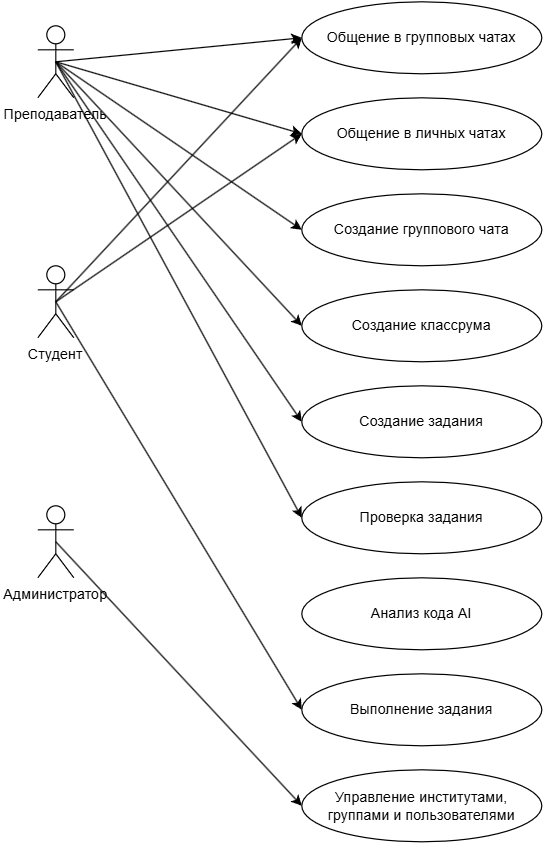
\includegraphics[width=0.5\linewidth]{static/useCaseDiagramm}
\caption{Диаграмма вариантов использования системы для различных ролей пользователей.}
\label{fig:usecasediagramm}
\end{figure}

\begin{figure}[h]
    \centering
    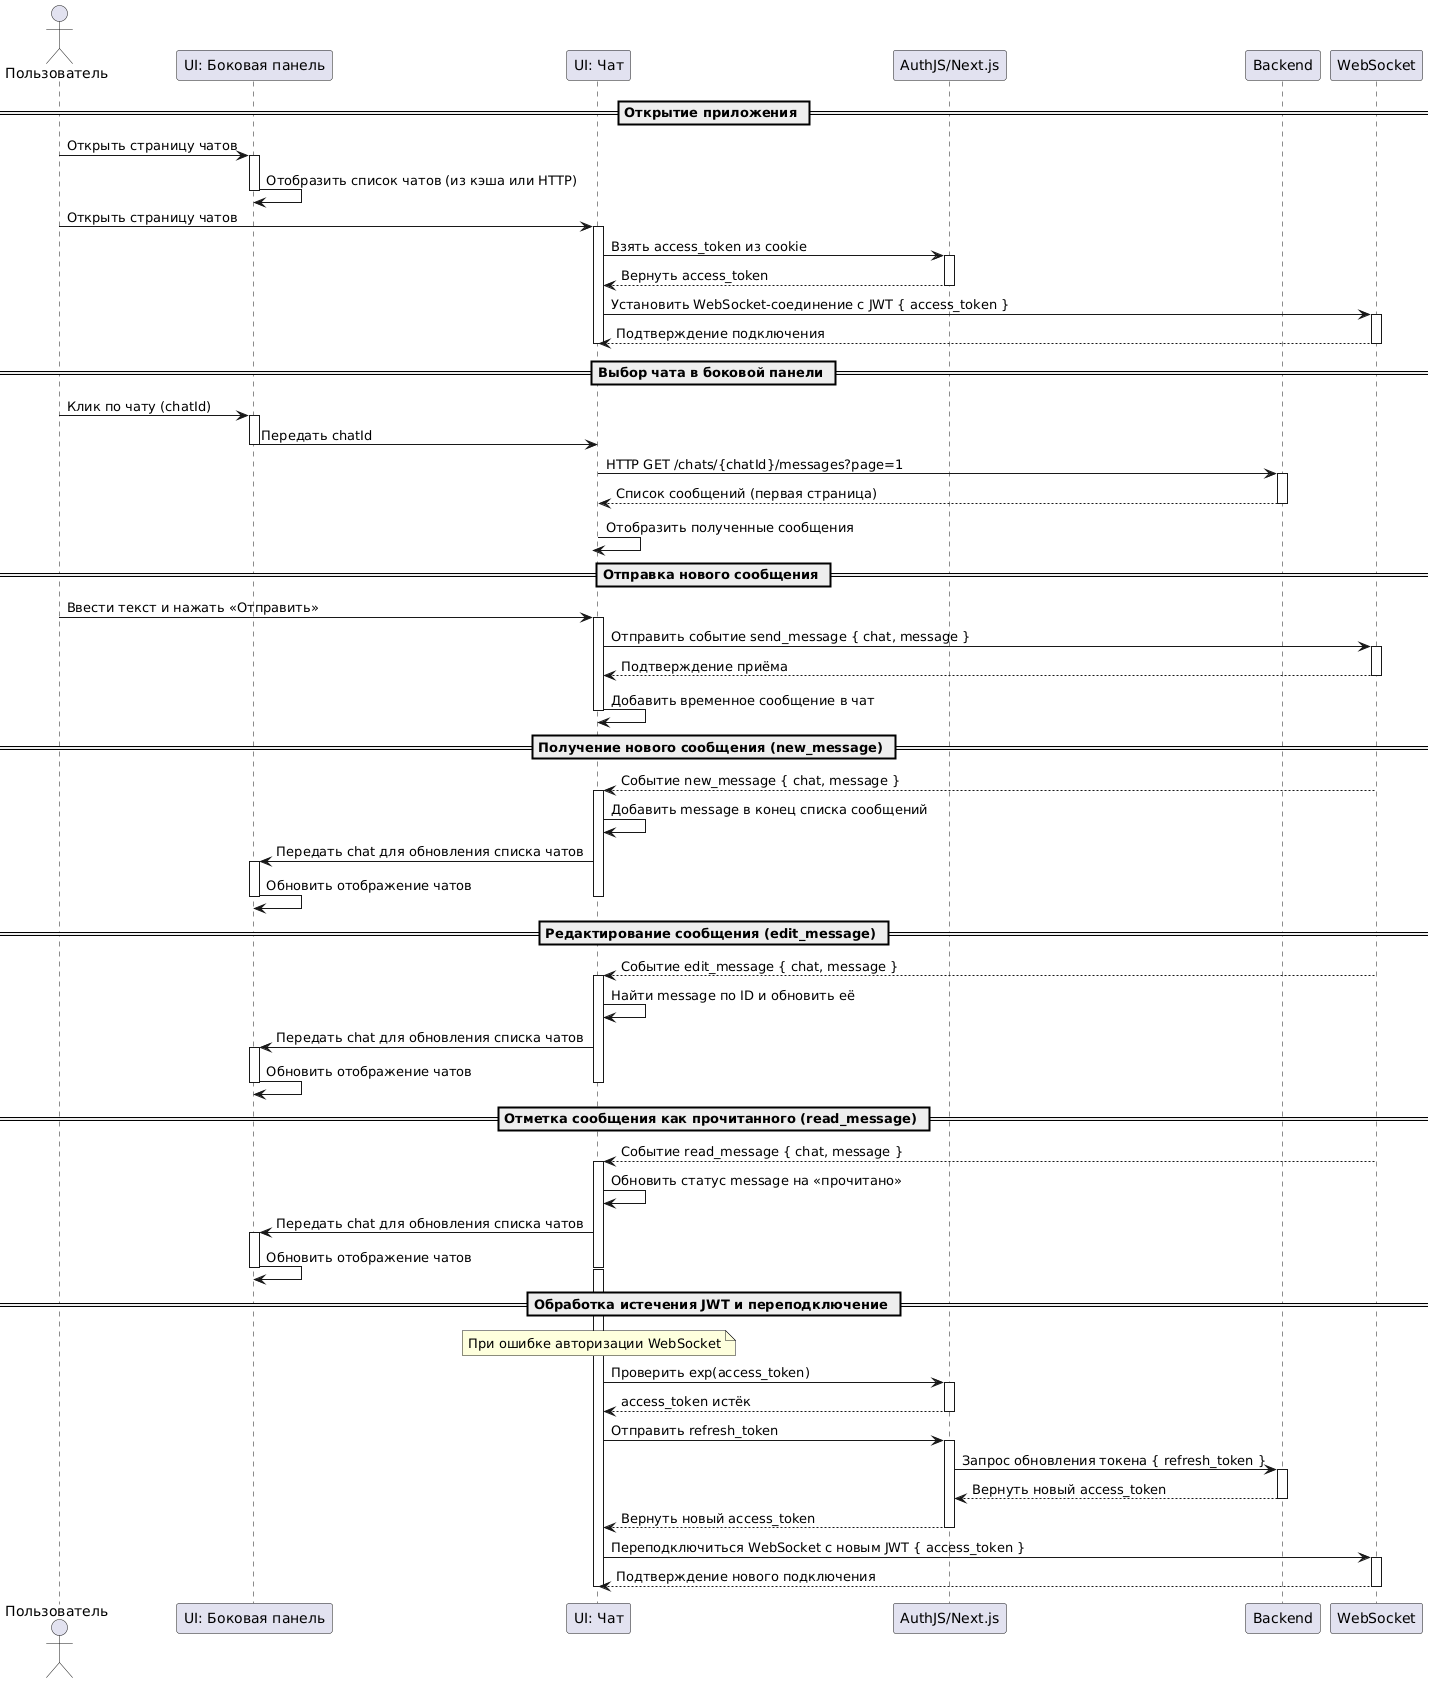
\includegraphics[width=0.9\textwidth]{static/diagrams/Chats.png}
    \caption{Схема взаимодействия клиента (UI: Боковая панель и UI: Чат), AuthJS (Next.js), севера и WebSocket протокола при работе модуля «Chats».}
    \label{fig:chats-flow}
\end{figure}


\begin{figure}[h]
    \centering
    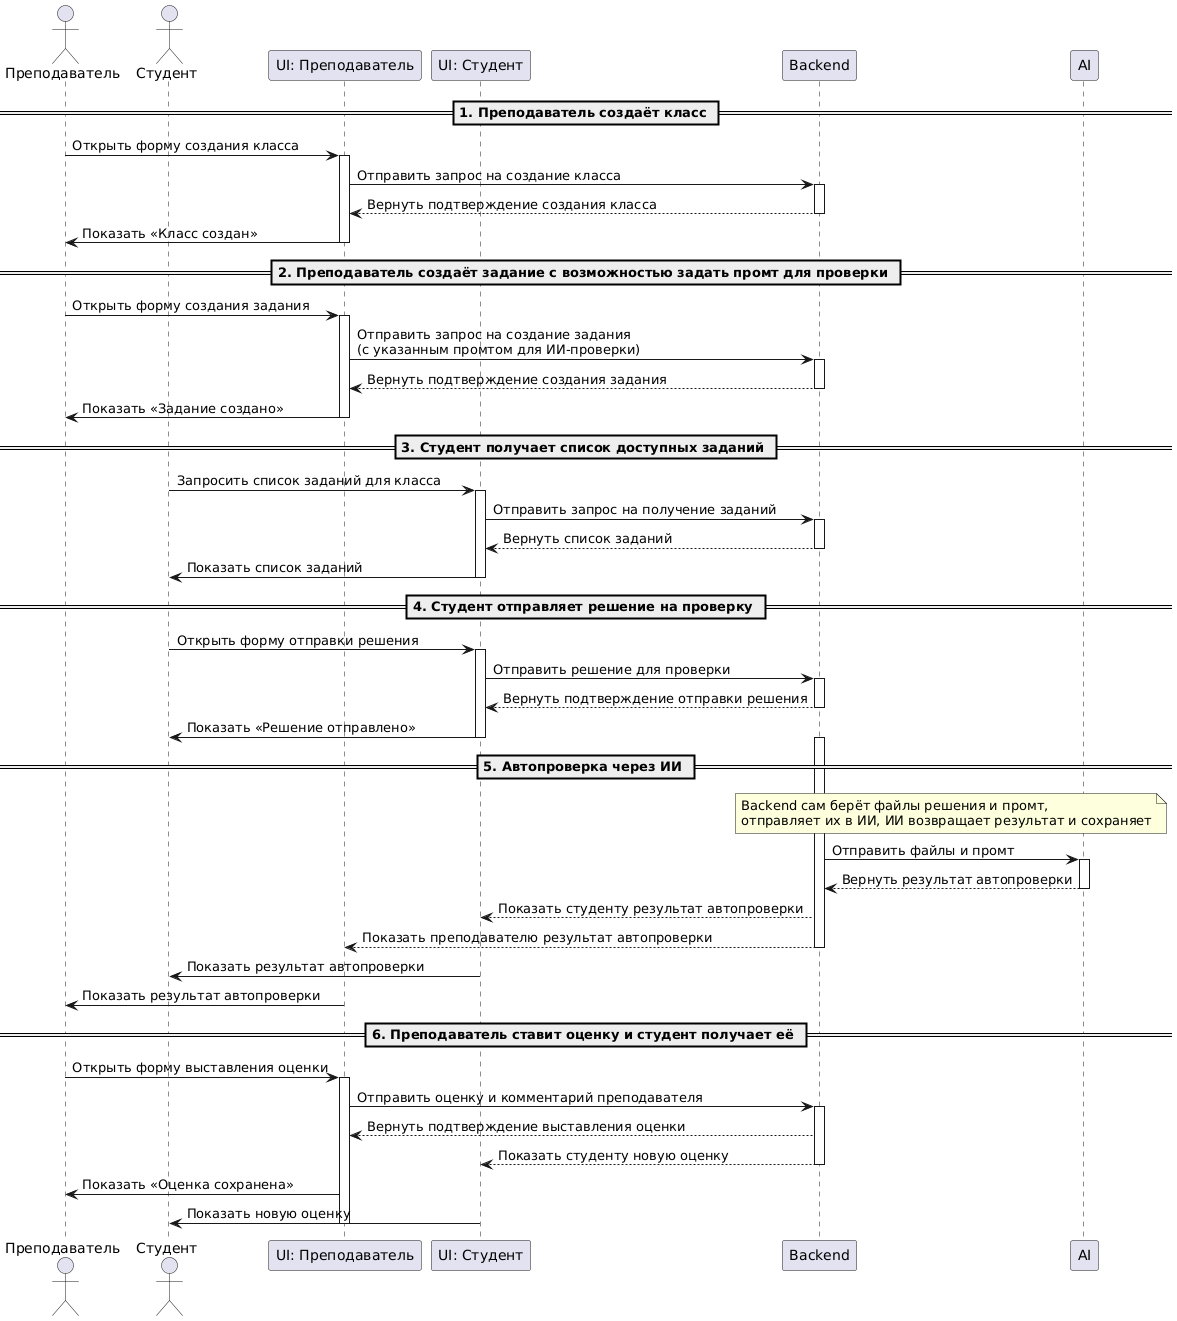
\includegraphics[width=0.9\textwidth]{static/diagrams/Classroom.png}
    \caption{Схема взаимодействия преподавателя, студента, и искуственного интелекта при работе с виртуальными классами}
    \label{fig:classroom-flow}
\end{figure}

  
\begin{figure}[h]
	\centering
	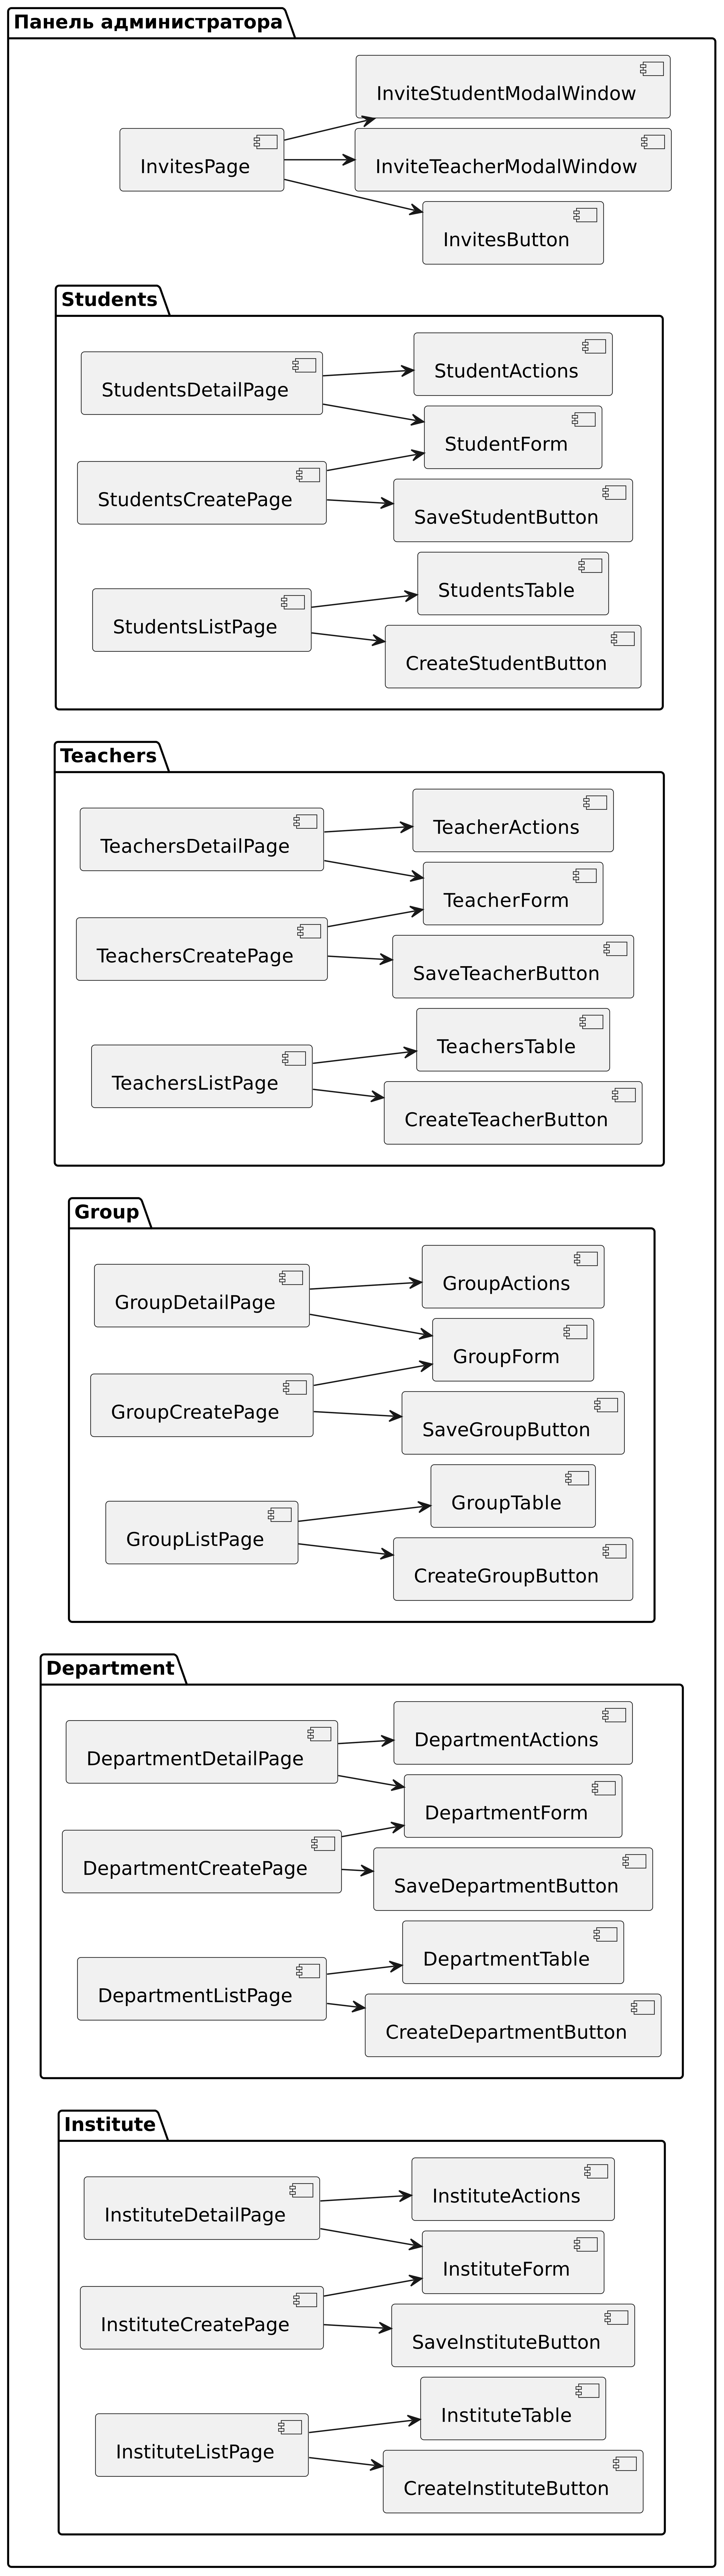
\includegraphics[width=0.4\textwidth]{static/diagrams/AdminComponentDiagram.png}
	\caption{Диаграмма компонентов административной панели}
	\label{fig:admin-components}
\end{figure}

\begin{figure}[h]
  \centering
  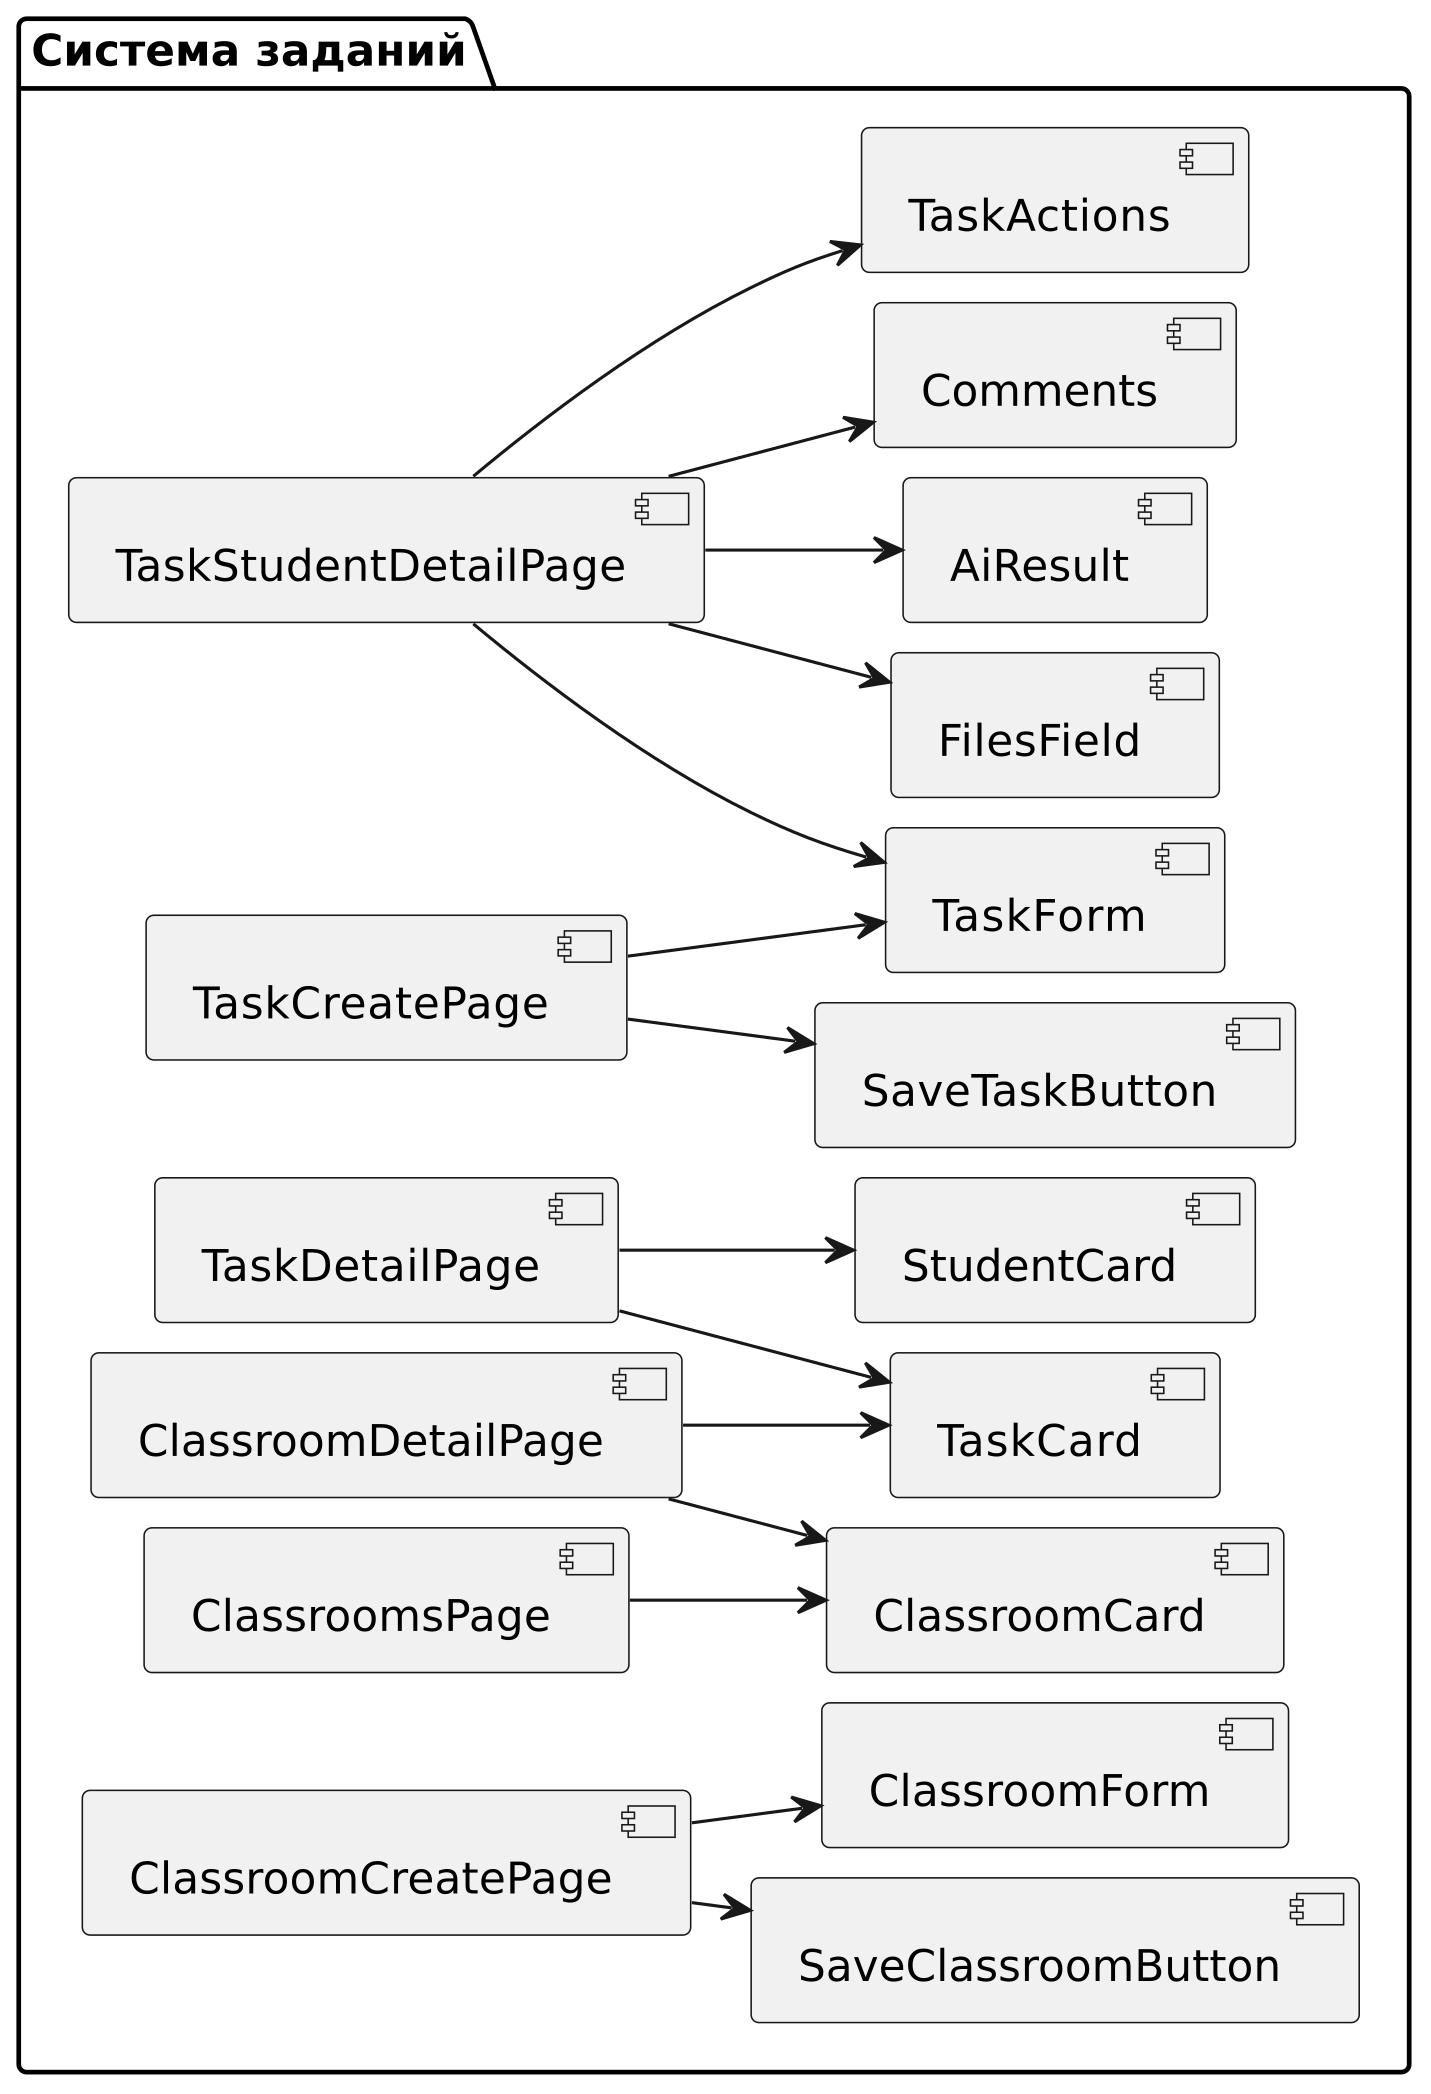
\includegraphics[width=0.7\textwidth]{static/diagrams/ClassroomComponentDiagram.png}
  \caption{Диаграмма компонентов системы заданий}
  \label{fig:classroom-components}
\end{figure}
 
\newpage
\clearpage
\ESKDthisStyle{formII}
\ESKDcolumnII{ПРИЛОЖЕНИЕ Б}
\begingroup
  % тут добавляем \centering в before-code
  \titleformat{\section}[block]
    {\normalfont\bfseries} % формат (оставляем обычный)
    {\thesection}          % номер секции
    {0.5em}                % отступ между номером и текстом
    {\centering}           % before-code: теперь центрируем
  \section*{ПРИЛОЖЕНИЕ Б}
\endgroup
\addcontentsline{toc}{section}{ПРИЛОЖЕНИЕ Б}
\begin{center}
\textbf{Фрагмент текста программы модуля административной панели}
\end{center}

\begin{lstlisting}
import {useEffect, useRef, useState} from "react";
import {UseIsErrorFieldIsErrorType} from "indicator-ui";
import {signIn} from "next-auth/react";
import {
    getInviteInfo,
    InviteStudentRequestBodyType,
    InviteTeacherRequestBodyType,
    LoginRequestType,
    registerStudent,
    registerTeacher,
    RegistrationQueryType,
    RegistrationStudentRequestBodyType,
    RegistrationTeacherRequestBodyType
} from "@/entities/Auth";
import {UseRegistrationPropsType} from "../types";

export function useRegistrationStudentAndTeacher<T extends typeof registerTeacher | typeof registerStudent>({
                                                                                                                inviteId,
                                                                                                                registrationRequest,
                                                                                                            }: UseRegistrationPropsType<T>) {
    type FormDataType = Parameters<T>[1]
    type InviteBodyType = T extends typeof registerTeacher ? InviteTeacherRequestBodyType : InviteStudentRequestBodyType
    const formDataRef = useRef<Omit<FormDataType, 'invite_id'> | undefined>(undefined)
    const [isError, setIsError] = useState<UseIsErrorFieldIsErrorType>([])
    const [initData, setInitData] = useState<InviteBodyType | null | undefined>({email: 'besmilev@gmail.com'} as anyтукт)

    useEffect(() => {
        const getInitData = async () => {
            let response
            if (inviteId) {
                response = await getInviteInfo({invite_id: inviteId}) as InviteBodyType
            } else {
                response = null
            }
            setInitData(response)
        }
        getInitData()
    }, [inviteId]);

    const onSubmit = async () => {
        const formData = formDataRef.current
        if (formData && inviteId) {
            // Пришлось заткнуть ts так как ему мозгов не хватает сопоставить тип T и функции,
            // а также из-за отсутствия полноценной типизации именно function
            const response = await registrationRequest({invite_id: inviteId}, {
                ...formData,
            } as unknown as (RegistrationQueryType & RegistrationTeacherRequestBodyType & RegistrationStudentRequestBodyType))

            if (response) {
                const loginData: LoginRequestType = {username: formData.email, password: formData.password}
                const loginResponse = await signIn("credentials", {
                    ...loginData,
                    redirect: false,
                })
                if (loginResponse.error) {
                    // Обработка ошибки аутентификации
                } else {
                    // Успешная аутентификации
                }
            }
        }
    }

    return {
        initData,
        onSubmit,
        isError,
        setIsError,
        formDataRef,
    }
}

export function CreateStudentsInvites({onClose}: { onClose?: () => void }) {
    const {onSend, inviteUrl, onCopy, onChangeFormData} = useCreateStudentInvites()

    return (
        <div className={InviteStyle.invite}>
            <MicroButton size={'28'}
                         color={'light'}
                         icon={<XCloseSVG/>}
                         additionStyles={InviteStyle.closeButton}
                         onClick={onClose}/>
            <h3 className={InviteStyle.header}>Пригласить студентов</h3>
            <div className={InviteStyle.form}>
                <FormBuilder onChange={onChangeFormData} schema={inviteStudentsScheme({})}/>
            </div>
            <Button size={'large'}
                    hierarchy={'primary'}
                    width={'fill'}
                    onClick={onSend}
                    text={'Сформировать ссылку'}/>
            <InputField labelText={'Ссылка'}
                        value={inviteUrl}
                        help={<Button size={'small'}
                                      onClick={onCopy}
                                      hierarchy={'secondary-color'}
                                      iconLeft={<Copy06SVG/>}/>}/>
        </div>
    )
}

export function CreateTeacherInvites({onClose}: { onClose?: () => void }) {
    const {onSend, onChangeFormData, inviteUrl, onCopy} = useCreateTeacherInvites()

    return (
        <div className={InviteStyle.invite}>
            <MicroButton size={'28'}
                         color={'light'}
                         icon={<XCloseSVG/>}
                         additionStyles={InviteStyle.closeButton}
                         onClick={onClose}/>
            <h3 className={InviteStyle.header}>Пригласить преподавателя</h3>
            <div className={InviteStyle.form}>
                <FormBuilder onChange={onChangeFormData} schema={inviteTeacherScheme()}/>
            </div>
            <Button size={'large'}
                    hierarchy={'primary'}
                    width={'fill'}
                    onClick={onSend}
                    text={'Сформировать ссылку'}/>
            <InputField labelText={'Ссылка'}
                        value={inviteUrl}
                        help={<Button size={'small'}
                                      hierarchy={'secondary-color'}
                                      onClick={onCopy}
                                      iconLeft={<Copy06SVG/>}/>}/>
        </div>
    )
}

export function AdminInvitesPage() {
    const [isActiveModalWindow, setIsActiveModalWindow] = useState<'teacher' | 'students' | undefined>(undefined)

    const isShow = () => {
        return isActiveModalWindow !== undefined
    }

    const setIsShow = (isShow: boolean) => {
        if (!isShow) {
            setIsActiveModalWindow(undefined)
        }
    }

    const getModalWindow = () => {
        switch (isActiveModalWindow) {
            case 'teacher':
                return <CreateTeacherInvites onClose={() => setIsActiveModalWindow(undefined)}/>
            case 'students':
                return <CreateStudentsInvites onClose={() => setIsActiveModalWindow(undefined)}/>
        }
    }

    return (
        <div className={AdminDetailPageStyle.AdminDetailPage}>
            <div className={clsx(AdminDetailPageStyle.content, AdminDetailPageStyle.fill, AdminDetailPageStyle.offWrapper)}>
                <h1 className={AdminDetailPageStyle.header}>Создание приглашений</h1>
                <ActionField title={'Пригласить преподавателя'}
                             subtitle={'Сформировать ссылку, по которой преподаватель может пройти регистрацию'}
                             onClick={() => setIsActiveModalWindow('teacher')}/>
                <ActionField title={'Пригласить студентов'}
                             subtitle={'Сформировать ссылку, по которой студенты могут пройти регистрацию'}
                             onClick={() => setIsActiveModalWindow('students')}/>
            </div>
            <BackgroundModalWindowWrapper isShow={isShow()}
                                          setIsShow={setIsShow}
                                          className={AdminDetailPageStyle.modalWindowWrapper}>
                {getModalWindow()}
            </BackgroundModalWindowWrapper>

        </div>
    )
}
\end{lstlisting}



\newpage
\clearpage
\ESKDthisStyle{formII}
\ESKDcolumnII{ПРИЛОЖЕНИЕ В}
\begingroup
  % тут добавляем \centering в before-code
  \titleformat{\section}[block]
    {\normalfont\bfseries} % формат (оставляем обычный)
    {\thesection}          % номер секции
    {0.5em}                % отступ между номером и текстом
    {\centering}           % before-code: теперь центрируем
  \section*{ПРИЛОЖЕНИЕ В}
\endgroup
\addcontentsline{toc}{section}{ПРИЛОЖЕНИЕ В}
\begin{center}
\textbf{Фрагмент текста программы модуля системы заданий}
\end{center}

\begin{lstlisting}
'use client'

import {Button, FormBuilder} from "indicator-ui";
import Link from "next/link";
import {ArrowNarrowLeftSVG} from "@/shared/assets";
import {ClassroomPostType} from "@/entities/Classroom";
import {ROUTES_CONFIG} from "@/features/Routing";
import {classroomScheme} from "@/features/Classrooms";
import {ClassroomCreatePageStyle} from '../styles'
import {useClassroomCreate} from "../hooks";

export function ClassroomCreatePage() {
    const {onChangeFormData, onSubmit} = useClassroomCreate()

    return (
        <div className={ClassroomCreatePageStyle.ClassroomCreatePage}>
            <Button hierarchy={'link-color'}
                    text={'Назад'}
                    iconLeft={<ArrowNarrowLeftSVG/>}
                    customComponent={<Link href={ROUTES_CONFIG.CLASSROOMS_PAGE}/>}/>
            <div className={ClassroomCreatePageStyle.content}>
                <FormBuilder<ClassroomPostType> schema={classroomScheme()} onChange={onChangeFormData}/>
                <Button size={'large'} width={'fill'} text={'Создать класс'} onClick={onSubmit}/>
            </div>
        </div>
    )
}

export function ClassroomDetailPage({id}: { id: number }) {
    const {list, classroom} = useClassroomDetail(id)

    if (list === undefined || classroom === undefined) {
        return 'Loading'
    }

    if (list === null || classroom === null) {
        return 'Error'
    }

    return (
        <div className={ClassroomDetailPageStyle.ClassroomDetailPage}>
            <ClassroomCard name={classroom.name}
                           description={classroom.description}
                           groupName={classroom.group.name}
                           width={'fill'}/>
            <Button size={'large'}
                    hierarchy={'secondary-color'}
                    text={'Добавить задание'}
                    width={'fill'}/>
            <div className={ClassroomDetailPageStyle.list}>
                {list.data.map((item, idx) => <TaskCard deadline={item.deadline}
                                                        name={item.name}
                                                        href={ROUTES_CONFIG.TASKS_DETAIL_SLUG_PAGE + item.id}
                                                        key={idx}/>)}
            </div>
            <PaginationComponent totalCount={list.total_count}/>
        </div>
    )
}

export function ClassroomsPage() {
    const {list} = useClassrooms()

    if (list === undefined) {
        return 'Loading...'
    }

    if (list === null) {
        return 'Error'
    }

    return (
        <div className={ClassroomsPageStyle.ClassroomsPage}>
            <div className={ClassroomsPageStyle.list}>
                {list.data.map((item, idx) => <ClassroomCard name={item.name}
                                                             description={item.description}
                                                             groupName={item.group.name}
                                                             avatar={item.avatar}
                                                             href={ROUTES_CONFIG.CLASSROOMS_DETAIL_SLUG_PAGE + item.id}
                                                             key={idx}/>)}
            </div>
            <PaginationComponent totalCount={list.total_count}/>
            <Button size={'large'}
                    width={'fill'}
                    hierarchy={'secondary-color'}
                    text={'Создать класс'}
                    customComponent={<Link href={ROUTES_CONFIG.CLASSROOMS_CREATE_PAGE}/>}/>
        </div>
    )
}
\end{lstlisting}


\newpage
\clearpage
\ESKDthisStyle{formII}
\ESKDcolumnII{ПРИЛОЖЕНИЕ Г}
\begingroup
  % тут добавляем \centering в before-code
  \titleformat{\section}[block]
    {\normalfont\bfseries} % формат (оставляем обычный)
    {\thesection}          % номер секции
    {0.5em}                % отступ между номером и текстом
    {\centering}           % before-code: теперь центрируем
  \section*{ПРИЛОЖЕНИЕ Г}
\endgroup
\addcontentsline{toc}{section}{ПРИЛОЖЕНИЕ Г}
\begin{center}
\textbf{Фрагмент текста программы модуля обмена сообщениями}
\end{center}

\begin{lstlisting}
import React, {forwardRef, useImperativeHandle, useRef} from "react";
import {v4 as uuidv4} from "uuid";
import {MessageInput, MessageInputRefType} from "@/shared/ui";
import {ChatSocketEmitType, GetMessageByIdResponseType} from "@/entities/Message";
import {MessageInputStyle} from "../../styles";
import {MessageInputPropsType, MessageInputRefType} from "../../types";

type SendMessageType = Parameters<ChatSocketEmitType['send_message']>[number];
type EditMessageType = Parameters<ChatSocketEmitType['edit_message']>[number];
type ReplayMessageDataType = GetMessageByIdResponseType['id']

type OnSendMessageType<ReplayMessageDataType> = Parameters<typeof MessageInput<ReplayMessageDataType>>[number]['onSend']
type OnEditMessageType<ReplayMessageDataType> = Parameters<typeof MessageInput<ReplayMessageDataType>>[number]['onEdit']
export const MessageInput = forwardRef<MessageInputRefType, MessageInputPropsType>((props, ref) => {
    const {
        curChat,
        sendMessage,
        editMessage,
    } = props
    const inputServicesRef = useRef<MessageInputRefType<ReplayMessageDataType>>(null);

    const onEditMessage: OnEditMessageType<ReplayMessageDataType> = async ({message}) => {
        if ((message.text || message.attachment?.length) && message.data) {
            const newMessage: EditMessageType = {
                id: message.data,
                text: message.text || '',
                attachments: message.attachment || [],
            }
            editMessage(newMessage)
            return true
        }
        return false
    }
    const onSendMessage: OnSendMessageType<ReplayMessageDataType> = async ({message, replayMessage}) => {
        if ((message.text || message.attachment?.length)) {
            // Генерируем uuid, потому что будем показывать сообщение сразу на фронте,
            // не дожидаясь ответа от бэка по socket
            const uuid = uuidv4();
            const newMessage: SendMessageType = {
                chat_id: curChat.id,
                text: message.text || '',
                attachments: message.attachment || [],
                reply_id: replayMessage?.data || null,
                local_id: uuid,
            }
            sendMessage(newMessage)
            return true
        }
        return false
    }

    const onEdit: MessageInputRefType['onEdit'] = (message) => {
        inputServicesRef.current?.editMessage({
            text: message.text,
            attachment: message.attachments,
            data: message.id,
        })
    }

    const onReplay: MessageInputRefType['onReplay'] = (message) => {
        inputServicesRef.current?.replayMessage({
            data: message.id,
            text: message.text,
            attachment: message.attachments,
        })
    }

    useImperativeHandle(ref, () => {
        return {
            onEdit,
            onReplay,
        }
    }, []);

    return (
        <div className={MessageInputStyle.MessageInput}>
            <MessageInput<ReplayMessageDataType> onSend={onSendMessage}
                                                 onEdit={onEditMessage}
                                                 ref={inputServicesRef}/>
        </div>
    )
})


export const MessageFeed = forwardRef<MessageFeedRefType, MessageFeedPropsType>((props, ref) => {
    const {
        curChat,
        onReplayMessage,
        onReadMessage,
        messages,
        onScrollTop,
        onScrollBottom,
        jumpToLastMessage,
        jumpToMessage,
        onEditMessage
    } = props;

    const {
        userId,
        SCROLL_ACCURACY,
        listRef,
        scrollToMessage,
        scrollToBottom,
        showScrollButton,
        onScroll,
        addFeedItemService,
        isFirstInGroup,
        isLastInGroup,
        saveScrollPosition,
        revertScrollPosition,
        blinkMessage,

        onChooseMessage,
        onReply,
        onEdit,
        chatActionsServiceRef,
    } = useMessageFeed(props)

    useImperativeHandle(ref, () => {
        return {
            scrollToBottom,
            scrollToMessage,
            saveScrollPosition,
            revertScrollPosition,
            blinkMessage,
        }
    }, []);

    if (!userId) {
        return <LoaderPage/>
    }

    return (
        <div className={MessageFeedStyle.MessageFeed}>
            <ChatActionsWindow ref={chatActionsServiceRef} onEdit={onEdit} onReplay={onReply}/>
            <ScrollProvider className={MessageFeedStyle.feed}
                            onScrollBottom={onScrollBottom}
                            onScrollTop={onScrollTop}
                            accuracy={SCROLL_ACCURACY}
                            onScroll={onScroll}
                            ref={listRef}>
                {messages.map((item, idx) => {
                        const id = getMessageId(item);
                        return <MessageFeedItem item={item}
                                                      curChat={curChat}
                                                      onReply={() => onReplayMessage(item)}
                                                      onEdit={() => onEditMessage(item)}
                                                      readMessage={() => onReadMessage(item)}
                                                      jumpToMessage={jumpToMessage}
                                                      firstInGroup={isFirstInGroup(idx)}
                                                      lastInGroup={isLastInGroup(idx)}
                                                      onChooseMessage={(event) => onChooseMessage(item, {
                                                          x: event.clientX,
                                                          y: event.clientY
                                                      })}
                                                      key={id}
                                                      ref={(node) => addFeedItemService(id, node)}/>
                    }
                )}
            </ScrollProvider>
            <div className={MessageFeedStyle.scrollButton}>
                {showScrollButton && <ChatScrollButton counter={curChat.unread_messages || undefined}
                                                       onClick={jumpToLastMessage}/>}
            </div>
        </div>
    )
})

export const ChatWidget = forwardRef<ChatWidgetRefType, ChatWidgetPropsType>((props, ref) => {
    const {
        curChat,
    } = props;

    const {
        messages,
        sendMessage,
        jumpToMessage,
        addNewMessage,
        changeMessage,
        feedServicesRef,
        jumpToLastMessage,
        editMessage,
        inputServicesRef,
        onReplayMessage,
        onReadMessage,
        onEditMessage,
        onScrollTop,
        onScrollBottom,
        testSkip,
    } = usesChatWidget(props);

    useImperativeHandle(ref, () => {
        return {
            addNewMessage,
            changeMessage,
        }
    }, []);

    if (messages === undefined) {
        return <LoaderPage/>
    }

    if (messages === null) {
        return 'Error'
    }

    return (
        <div className={sChatWidgetStyle.sChatWidget}>
            <div className={sChatWidgetStyle.testSkip}>{testSkip}</div>
            <div className={sChatWidgetStyle.messageList}>
                <MessageFeed messages={messages}
                                   curChat={curChat}
                                   jumpToMessage={jumpToMessage}
                                   jumpToLastMessage={jumpToLastMessage}
                                   onReadMessage={onReadMessage}
                                   onEditMessage={onEditMessage}
                                   onScrollTop={onScrollTop}
                                   onScrollBottom={onScrollBottom}
                                   onReplayMessage={onReplayMessage}
                                   ref={feedServicesRef}/>
            </div>
            <MessageInput curChat={curChat}
                                editMessage={editMessage}
                                sendMessage={sendMessage}
                                ref={inputServicesRef}/>
        </div>
    )
})

\end{lstlisting}
